\documentclass[12pt]{article}
\usepackage{amsmath}
\usepackage{graphicx}
\usepackage{hyperref}
\usepackage[utf8]{inputenc}
\usepackage{geometry}
\usepackage{mathtools}
\usepackage{empheq}
\usepackage{listings}
\usepackage{xcolor}
\usepackage{minted}
\definecolor{LightGray}{gray}{0.9}

\graphicspath{ {./} }
\geometry{margin=0.75in}

\title{CHEN 364 HW 2}
\author{Mark Levchenko}
\date{January 2023}

\begin{document}

\begin{enumerate}
% Problem 1 %%%%%%%%%%%%%%%%%%%%%%%%%%%%%%%%%%%%%%%%%%
\newpage
    \item Problem 1
    \begin{enumerate}
        \item
        \begin{align*}
            \intertext{Rate law:}
            \Aboxed{-r_A = k C_A C_B}
        \end{align*}
        \item
        \begin{align*}
            \intertext{Rate law:}
            \intertext{Catalyst k and $r_A$}
            \Aboxed{-r_A' &= k' P_A P_B}
        \end{align*}
        \item
        \begin{align*}
            \intertext{Rate law:}
            \Aboxed{-r_A = k C_A}
        \end{align*}
        \item
        \begin{align*}
            \intertext{Rate law:}
            \Aboxed{-r_A = k}
        \end{align*}
    \end{enumerate}

    The fourth rate law is strange because it is zeroth order. It does not make sense for a reaction to be independent of the concentration of any reactants. Why would a reaction be occurring if the concentration of the reactants is zero?

% Problem 2 %%%%%%%%%%%%%%%%%%%%%%%%%%%%%%%%%%%%%%%%%%
\newpage
    \item Problem 2
    \begin{equation*}
        \mathrm{A} \rightarrow \mathrm{B} + \mathrm{C}
    \end{equation*}
    \begin{align*}
        -r_A &= k C_A \\
        C_A &= C_{A0} (1 - X) \\
        \frac{F_{A0}}{-r_A} &= \frac{v_0 C_{A0}}{k C_{A0} (1 - X)} \\
        \frac{F_{A0}}{-r_A} &= \frac{v_0 }{k (1 - X)} \\
    \end{align*}

    Plot:
    
    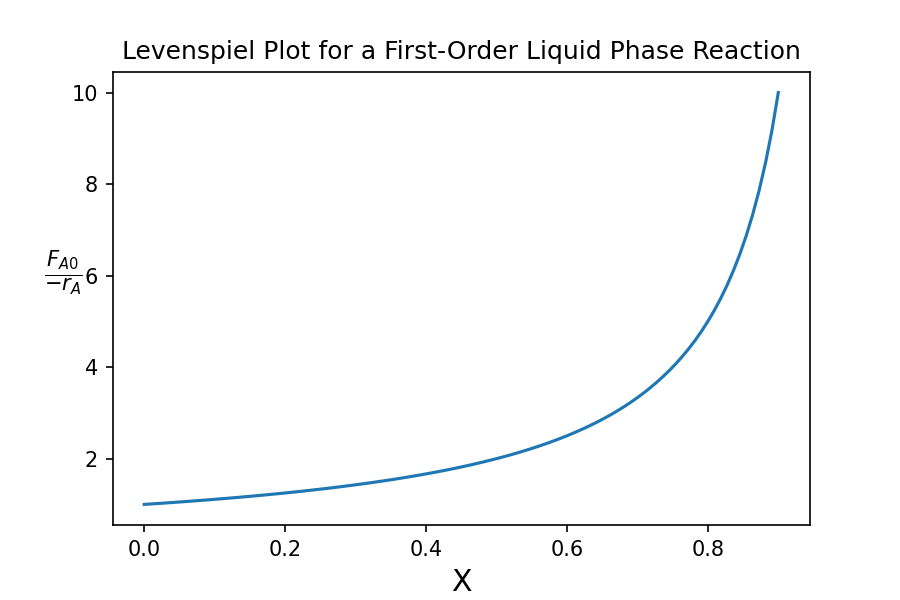
\includegraphics{CHEN364_HW2_P2_fig.png}


% Problem 3 %%%%%%%%%%%%%%%%%%%%%%%%%%%%%%%%%%%%%%%%%%
\newpage
    \item Problem 3
    \begin{equation*}
        \mathrm{A} + \mathrm{B} \rightarrow \mathrm{C}
    \end{equation*}
    \begin{align*}
        \intertext{CSTR design equation:}
        V_{CSTR} &= \frac{X F}{-r_A} \\
        V_{CSTR} &= \frac{X v_0 C_{A0}}{-r_A} \\
        \frac{V_{CSTR}}{v_0} &= \frac{X C_{A0}}{-r_A} \\
        \tau &= \frac{X C_{A0}}{-r_A} \\
        \intertext{Elementary rate law:}
        -r_A &= k C_A C_B \\
        C_A &= C_{A0} (1 - X) \\
        C_B &= C_{A0} \left( \frac{C_{B0}}{C_{A0}} - \frac{1}{1} X \right) \\
        -r_A &= k C_{A0}^2 (1 - X) \left( \frac{C_{B0}}{C_{A0}} - X \right) \\
        \tau &= \frac{X C_{A0}}{k C_{A0}^2 (1 - X) \left( \frac{C_{B0}}{C_{A0}} - X \right)} \\
        \tau &= \frac{X}{k C_{A0} (1 - X) \left( \frac{C_{B0}}{C_{A0}} - X \right)} \\
        X &= 0.9 \\
        C_{A0} &= 16.3 \\
        C_{B0} &= 55.5 \\
        k &= 0.01 \\
        \intertext{At 300K:}
        \tau &= \frac{0.9}{0.01 \cdot 16.3 \cdot (1 - 0.9) \left( \frac{55.5}{16.3} - 0.9 \right)} \\
        \Aboxed{\tau &= 21.96 \mathrm{s}} \\
        \intertext{At 350K:}
        k' &= k \exp{\frac{E}{R}\left( \frac{1}{T_1} - \frac{1}{T_2} \right)} \\
        E &= 12500 \cdot 4.184 \\
        T_1 &= 300 \\
        T_2 &= 350 \\
        R &= 8.314 \\
        \tau &= \frac{0.9 \cdot (1 - 0.9)}{0.01 \cdot \exp{\frac{12500 \cdot 4.184}{8.314}\left( \frac{1}{300} - \frac{1}{350} \right)} \cdot 16.3 \cdot (1 - 0.9) \left( \frac{55.5}{16.3} - 0.9 \right)} \\
        \Aboxed{\tau &= 1.098 \mathrm{s}} \\
        \intertext{Reactor volume:}
        V &= v_0 \tau \\
        v_0 &= 200 \\
        \intertext{At 300K:}
        V &= 200 \cdot 21.96 \\
        \Aboxed{V &= 4392 \mathrm{L}} \\
        \intertext{At 350K:}
        V &= 200 \cdot 1.098 \\
        \Aboxed{V &= 219.6 \mathrm{L}}
    \end{align*}

% Problem 4 %%%%%%%%%%%%%%%%%%%%%%%%%%%%%%%%%%%%%%%%%%
\newpage
    \item Problem 4
    \begin{equation*}
        \frac{3}{2} \mathrm{A} + \frac{1}{2} \mathrm{B} \rightarrow \mathrm{C}
    \end{equation*}
    \begin{equation*}
        \mathrm{A} + \frac{1}{3} \mathrm{B} \rightarrow \frac{2}{3} \mathrm{C}
    \end{equation*}
    \begin{enumerate}
        \item Stoichiometric table:
    
        \begin{tabular}{c c c c}
            \hline
            Species & Initial & Change & Final \\
            \hline
            A & $F_{A0}$ & $-X$ & $F_{A0} (1 - X) $ \\
            B & $F_{B0}$ & $- \frac{1}{3} X$ & $F_{A0} (\Theta_{B} - \frac{1}{3} X) $ \\
            C & $F_{C0}=0$ & $\frac{2}{3} X$ & $F_{A0} (\Theta_{C} + \frac{2}{3} X) $ \\
            \hline
        \end{tabular}

        \item
        \begin{align*}
            \delta &= \frac{2}{3} - \frac{1}{3} - 1 \\
            \Aboxed{\delta &= -\frac{2}{3}} \\
            y_{A0} &= 0.5 \\
            y_{B0} &= 0.5 \\
            \epsilon &= 0.5 \cdot -\frac{2}{3}  \\
            \Aboxed{\epsilon &= -\frac{1}{3}}  \\
            P_{A0} &= 8.2 \mathrm{atm} = 830.865 \mathrm{kPa} \\
            C_{A0} &= \frac{P_{A0}}{RT} \\
            T &= 227 ^\circ\mathrm{C} = 500.15 \mathrm{K} \\
            C_{A0} &= \frac{830.865}{8.314 \cdot 500.15} \\
            \Aboxed{C_{A0} &= 0.2} \\
            C_A &= C_{A0} \left[ \frac{1 - X}{1 + \epsilon X} \right] \\
            C_A &= 0.3 \cdot \left[ \frac{1 - 0.6}{1 - \frac{1}{3} \cdot 0.6} \right] \\
            \Aboxed{C_A &= 0.1} \\
            C_C &= C_{A0} \left[ \frac{\Theta_C - \frac{2}{3} X}{1 + \epsilon X} \right] \\
            C_C &= 0.2 \left[ \frac{0 + \frac{2}{3} \cdot 0.6}{1 - \frac{1}{3} \cdot 0.6} \right] \\
            \Aboxed{C_C &= 0.1}
        \end{align*}

        \newpage
        \item
        \begin{align*}
            \intertext{Constant volumetric flow rate flow reactor:}
            -r_A &= k C_A^{\frac{3}{2}} C_B^{\frac{1}{2}} \\
            C_A &= C_{A0} \left[ \frac{1 - X}{1 + \epsilon X} \right] \frac{P}{P_0} \frac{T_0}{T} \\
            C_B &= C_{A0} \left[ \frac{\Theta_B - \frac{1}{3} X}{1 + \epsilon X} \right] \frac{P}{P_0} \frac{T_0}{T} \\
            \frac{P}{P_0} &= \frac{T_0}{T} \\
            C_A &= C_{A0} \left[ \frac{1 - X}{1 + \epsilon X} \right] \\
            C_B &= C_{A0} \left[ \frac{\Theta_B - \frac{1}{3} X}{1 + \epsilon X} \right] \\
            C_{A0} &= C_{B0} \\
            \Theta_B &= 1 \\
            C_B &= C_{A0} \left[ \frac{1 - \frac{1}{3} X}{1 + \epsilon X} \right] \\
            -r_A &= k \left( C_{A0} \left[ \frac{1 - \frac{1}{3} X}{1 - \frac{1}{3} X} \right] \right)^{\frac{1}{2}} \left( C_{A0} \left[ \frac{1 - X}{1 - \frac{1}{3} X} \right] \right)^{\frac{3}{2}} \\
            -r_A &= k C_{A0}^2 \left( \frac{1 - X}{1 - \frac{1}{3} X} \right)^{\frac{3}{2}} \\
            -r_A &= 40 \cdot 0.2^2 \left( \frac{1 - X}{1 - \frac{1}{3} X} \right)^{\frac{3}{2}} \\
            \Aboxed{-r_A &= 1.6 \cdot \left( \frac{1 - X}{1 - \frac{1}{3} X} \right)^{\frac{3}{2}}}
        \end{align*}


        \item
        \begin{align*}
            \intertext{PFR design equation:}
            F_{A0} \frac{dX}{dV} &= -r_A \\
            -r_A &= k C_{A0}^2 \left( \frac{1 - X}{1 - \frac{1}{3} X} \right)^{\frac{3}{2}} \\
            F_{A0} \frac{dX}{dV} &= k C_{A0}^2 \left( \frac{1 - X}{1 - \frac{1}{3} X} \right)^{\frac{3}{2}} \\
            \int_0^V dV &= \frac{F_{A0}}{k C_{A0}^2} \int_0^X \left( \frac{1 - X'}{1 - \frac{1}{3} X'} \right)^{-\frac{3}{2}} dX' \\
            F_{A0} &= 100 \\
            k &= 40 \\
            C_{A0} &= 0.2 \\
            X &= 0.6 \\
        \end{align*}

        \newpage
        Evaluate the integral with the following code:
\begin{minted}[
framesep=2mm,
baselinestretch=1.2,
bgcolor=LightGray,
fontsize=\footnotesize,
breaklines,
]{python}
import numpy as np
import matplotlib.pyplot as plt
from scipy.integrate import solve_ivp, trapezoid

# function inside integral
def P_4_d_diff(x):
  return ( (1 - x) / (1 - x / 3) ) ** (-3 / 2)

# constants
F_A0 = 100
k = 40
C_A0 = 830.865 / 8.314 / 500.15 # = 0.2

# conversion values array
X = np.linspace(0, 0.6, 1000)

# evaluate innner function at X
dV = P_4_d_diff(X)

# analytical integral
V = trapezoid(dV, X) * F_A0 / k / C_A0 ** 2
print(V)
# Aggie Honor Code: An Aggie does not lie, cheat, or steal or tolerate
# those who do.
# I certify that this work is my own and not the work of another.
#
# Name: Mark Levchenko
# Assignment #: HW 2
# Question #: 4d
\end{minted}

        Output:
        \begin{equation*}
            \boxed{V_{\mathrm{PFR}} = 59.91 \mathrm{L}}
        \end{equation*}
        
    \end{enumerate}




    
\end{enumerate}

\end{document}
